\documentclass{article}
\usepackage{qilin}
\tikzstyle{process} = [rectangle, rounded corners, minimum width=1.5cm, minimum height=0.5cm,align=center, draw=black, fill=gray!30, auto]
\title{PHY293: Tutorial Problems \\ \textbf{Tutorial 1 Solutions}}
\author{QiLin Xue}
\date{Fall 2021}
\usepackage{mathrsfs}
\usetikzlibrary{arrows}
\begin{document}

\maketitle
\begin{enumerate}
    \item \begin{enumerate}
        \item The angular frequency is $$\boxed{\omega = \sqrt{\frac{k}{m}} = 5\text{ rad/s}}$$
        \item The total mechanical energy of the system is equal to the potential energy at maximum compression: $$\boxed{E = \frac{1}{2}kA^2 = 0.36 \text{ J}}.$$
        \item Using conservation of energy, we have
        \begin{equation*}
            E = \frac{1}{2}mv^2 + \frac{1}{2}kx(0)^2.
        \end{equation*}
        We know everything except $v$, so solving for it gives $v = 0.566 \text{ m/s}.$ We want velocity so the answer is $$\boxed{\vec{v} = 0.566\text{ m/s [right]}}.$$
        \item We have $x(t)=A\sin(\omega t + \phi).$ Using the initial condition $x(0)=-0.04\text{ m},$ we have $-0.333 = \sin(\phi).$ We get two solutions: $\phi = -19.47^\circ$ and $\phi = 199.5^\circ.$ We want $v(0) = A\omega\cos(\phi)> 0,$ so the right solution is $\boxed{\phi=19.47^\circ}$.
        \item The spring will reach equilibrium when $\sin(\omega t+\phi)=0,$ or when $\omega t + \phi = 0$. This occurs after a time $$\Delta t = \frac{-\phi}{\omega} = 0.0680 \text{ s}.$$
        Since the spring is symmetric across equilibrium, it takes another $\Delta t$ seconds to reach $+0.040\text{ m}$, so the time at which it first reaches here is $$\boxed{t_1 = 2\Delta t = 0.136\text{ s}.}$$
        The period is $T=\frac{2\pi}{\omega} = 1.257\text{ s}$, so the time at which the block reaches this location a second time (i.e. on the way back) is: 
        $$\boxed{t_2 = T/2 = 0.628\text{ s}}.$$
    \end{enumerate}
    \item The velocity function is given by $v(t)=A\omega \cos(\omega t + \phi).$ The maximum speed is $A\omega = 2\text{ cm/s},$ and $v(0)=-1$, so we have $-1=2\cos(\phi)$. Solving for $\phi$ gives $\phi=120^\circ$ and $\phi=240^\circ$.
    
    The mass is travelling to the left and is about to reach maximum elongation, so the position $x(t)=A\sin(\phi)$ is negative. Therefore, we have $\boxed{\phi=240^\circ}$.

    \newpage
    \item \textbf{System 1:} The angular frequency is $\omega = \sqrt{\frac{k_a}{m}}.$ 
    
    \textbf{System 2:} Suppose the block is moved a distance $x$ from equilibrium. Then the equation of motion (from $F=ma$) is: 
    $$ma = -k_bx + (-k_bx) = -2k_bx.$$
    Therefore, the effective spring constant is $2k_b$ and the angular frequency is $\omega = \sqrt{\frac{2k_b}{m}}.$

    \textbf{System 3:} We claim that the effective spring constant is $\frac{k_c}{2}$. There are three ways to see this: 
    \begin{itemize}
        \item \textit{Method 1:} The springs are identical, so if one spring stretches by $\Delta x/2$, then the other spring will also stretch by $\Delta x/2$, resulting in a net stretch of $\Delta x$. Therefore, when the mass moves a distance $x$, it only experiences a force of $-k(x/2).$
        \item \textit{Method 2:} We can view this as one long spring. Recall from CIV102 that the spring constant is $k = \frac{EA}{L}$, where $E$ is the Young's Modulus, $A$ is the cross sectional area, and $L$ is the length. We're not changing $E$ or $A$, but by doubling $L$, we are halving $k.$
        \item \textit{Method 3:} Let the mass move a distance $d$ and let the spring attached to it get stretched a distance $\Delta x_1$, and let the spring attached to the wall get stretched a distance $\Delta x_2$. We want to relate $\Delta x_1$ and $\Delta x_2$. From Newton's third law, we have 
        \begin{equation*}
            k_c\Delta x_1 = k_c \Delta x_2 \implies \Delta x_1 = \Delta x_2
        \end{equation*}
        and we can continue with the same argument as method 1. However, this is a bit more general and can be used when the spring constants are not equal.
    \end{itemize}
    The angular frequency is then $\omega = \sqrt{\frac{k_c}{2m}}$. These frequencies are all equal, so we have 
    \begin{equation*}
        \sqrt{\frac{k_a}{m}} = \sqrt{\frac{2k_b}{m}} = \sqrt{\frac{k_c}{2m}} \implies k_a = 2k_b = k_c/2
    \end{equation*}
    which leads to the desired ratio of 
    \begin{equation*}
        \boxed{k_a:k_b:k_c = 1:1/2:2.}
    \end{equation*}
    \item We can consider the forces acting on it. There is a gravitational force $mg$ downwards and a normal force $N$ upwards. The mass will loss contact with the platform when $N=0$, i.e. when the acceleration of the block is $g$.
    
    The platform moves with a position $y(t) = A\sin(\omega t)$ where $\omega = 2\pi f = 15.7 \text{ rad/s}.$ Then the acceleration is $a(t) = A\omega^2\sin(\omega t)$ and reaches a maximum value of $A\omega^2.$ This is equal to $g$ when $$\boxed{A = g/\omega^2 = 0.04\text{ m}}.$$
    \item \begin{enumerate}
        \item We want to find an amplitude $A$ such that
        \begin{equation}
            10\cos(\omega t) = 10\cos(\omega t+ 1) + A\cos(\omega t + \phi),
        \end{equation}
        or alternatively:
        \begin{align*}
            10\cos(\omega t) - 10\cos(\omega t+ 1)  &= 10 \left(-2\sin\left((\omega t + \omega t + 1)/2\right)\cos\left((\omega t - \omega t - 1)/2\right)\right) \\ 
            &= -20\sin(\omega t + 0.5)\sin(-1/2) \\ 
            &= 9.59\sin(\omega t + 0.5)
        \end{align*}
        where we used the difference in cosine formula. Therefore, the magnitude is $\boxed{|I_2|=9.59\text{ A}}$. There is actually a nice geometric interpretation of this using phasors. We want:
        \begin{center}
            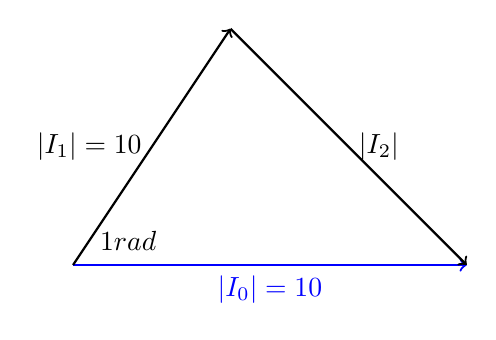
\begin{tikzpicture}
                \draw[blue,thick,->] (0,0) -- (5,0) node[midway,below] {$|I_0|=10$};
                \draw[thick,->] (0,0) node[shift={(0.7,0.3)}] {$1 \text{ rad}$} -- (2,3) node[midway,left] {$|I_1|=10$};
                \draw[thick,->] (2,3) -- (5,0) node[midway,right] {$|I_2|$};
            \end{tikzpicture}
        \end{center}
        The sum of the two phasors $I_1+I_2$ needs to be horizontal (which represents no phase shift), and we can determine this using cosine law: 
        \begin{equation}
            |I_2| = \sqrt{10^2+10^2-2(10)(10)\cos(1)} = 9.59.
        \end{equation}
        \item Using the same idea, note that the smallest $|I_2|$ such that the sum of the two phasors lie on the horizontal line is if $I_2$ is perpendicular to $I_0$, in which we can use standard trigonometry: 
        \begin{equation}
            \boxed{I_2 = I_1\sin(1) = 8.41 \text{ A}}.
        \end{equation}
    \end{enumerate}
    \item The period does not depend on the mass, so we have 
    \begin{center}
        \begin{tikzpicture}
        \begin{axis}[
        legend pos=outer north east,
        title=Period Dependance on Mass,
        axis lines = box,
        xlabel = $m$,
        ylabel = $T$,
        yticklabels={,,},
        xticklabels={,,},
        ymin = 0,
        ymax = 2,
        variable = t,
        trig format plots = rad,
        ]
        \addplot [
            domain=0:10,
            samples=70,
            color=blue,
            ]
            {1};
        \end{axis}
        \end{tikzpicture}
    \end{center}
    The period depends on length as $T \propto \sqrt{\ell}$, so we have: 
    \begin{center}
        \begin{tikzpicture}
        \begin{axis}[
        legend pos=outer north east,
        title=Period Dependance on Length,
        axis lines = box,
        xlabel = $\ell$,
        ylabel = $T$,
        yticklabels={,,},
        xticklabels={,,},
        ymin = 0,
        ymax = 2,
        variable = t,
        trig format plots = rad,
        ]
        \addplot [
            domain=0:10,
            samples=200,
            color=blue,
            ]
            {sqrt(x)};
        \end{axis}
        \end{tikzpicture}
    \end{center}

    \newpage
    \item \begin{enumerate}
        \item Using trigonometry, we have
        \begin{equation}
            \boxed{\theta = \sin^{-1}\left(\frac{0.0350}{0.750}\right) = 2.67^\circ}
        \end{equation}
        The small angle approximation can be used.

        \textit{Note:} To be more complete, using this $\theta$ results in approximately a $0.04\%$ error. This is much less error than possible uncertainties in the length and position measurements.
        \item The initial height (measured from the top) is 
        \begin{equation}
            h = \sqrt{0.750^2-0.0350^2} = 0.74918 \text{ m}.
        \end{equation}
        so there is a height difference of $\Delta h = 0.000817 \text{ m}$ between the maximum and lowest point. Energy conservation tells us the maximum speed is 
        \begin{equation}
            \boxed{v=\sqrt{2g\Delta h}=0.127\text{ m/s}}.
        \end{equation}
        \item This is a fourth of the period, so the time to reach this speed is 
        \begin{equation}
            \boxed{t=T/4 = \frac{1}{4} \cdot 2\pi\sqrt{\frac{\ell}{g}} = 0.434 \text{ s}.} 
        \end{equation}
    \end{enumerate}
    \item \begin{enumerate}
        \item The relationship between a conservative force and potential energy is 
        \begin{equation}
            F = -\frac{\dd{U}}{\dd{x}}
        \end{equation}
        Applying this, we get 
        \begin{equation}
            \boxed{F = \frac{6a}{x^7} - \frac{12b}{x^{13}}}.
        \end{equation}
        \item Equilibrium occurs when $F=0$, or when: 
        \begin{equation}
            \frac{6a}{x^7} = \frac{12b}{x^{13}} \implies \boxed{x_0 = \left(\frac{2b}{a}\right)^{1/6}}.
        \end{equation}
        \item The angular frequency at equilibrium is equal to 
        \begin{equation}
            \omega = \sqrt{\frac{U''(x)}{m}} = \sqrt{\frac{F'(x)}{m}}.
        \end{equation}
        Taking the derivative again, we get
        \begin{equation}
            F'(x) = -\frac{6a}{x^7}\frac{7}{x}+\frac{12b}{x^{13}} \frac{13}{x}.
        \end{equation}
        Letting $\frac{6a}{x^7} = \frac{12b}{x^{13}}$, we have: 
        \begin{align*}
            F'(x_0) &= -\frac{6a}{x_0^7}\frac{7}{x_0}+\frac{6a}{x_0^7} \frac{13}{x_0} \\ 
            &= \frac{6a}{x_0^6}\left(\frac{13}{x_0^2}-\frac{7}{x_0^2}\right) \\ 
            &= \frac{6a}{x_0^6}\left(\frac{6}{x_0^2}\right)
        \end{align*}
        Letting $x_0=\left(\frac{2b}{a}\right)^{1/6}$ and substituting this in, we have
        \begin{equation}
            \boxed{F'(x_0) = 36a \frac{a}{2b}\left(\frac{a}{2b}\right)^{1/3}=36a\left(\frac{a}{2b}\right)^{4/3}.}
        \end{equation}
    \end{enumerate}
\end{enumerate}
\end{document}